\documentclass{article}\usepackage[]{graphicx}\usepackage[]{color}
%% maxwidth is the original width if it is less than linewidth
%% otherwise use linewidth (to make sure the graphics do not exceed the margin)
\makeatletter
\def\maxwidth{ %
  \ifdim\Gin@nat@width>\linewidth
    \linewidth
  \else
    \Gin@nat@width
  \fi
}
\makeatother

\definecolor{fgcolor}{rgb}{0.345, 0.345, 0.345}
\newcommand{\hlnum}[1]{\textcolor[rgb]{0.686,0.059,0.569}{#1}}%
\newcommand{\hlstr}[1]{\textcolor[rgb]{0.192,0.494,0.8}{#1}}%
\newcommand{\hlcom}[1]{\textcolor[rgb]{0.678,0.584,0.686}{\textit{#1}}}%
\newcommand{\hlopt}[1]{\textcolor[rgb]{0,0,0}{#1}}%
\newcommand{\hlstd}[1]{\textcolor[rgb]{0.345,0.345,0.345}{#1}}%
\newcommand{\hlkwa}[1]{\textcolor[rgb]{0.161,0.373,0.58}{\textbf{#1}}}%
\newcommand{\hlkwb}[1]{\textcolor[rgb]{0.69,0.353,0.396}{#1}}%
\newcommand{\hlkwc}[1]{\textcolor[rgb]{0.333,0.667,0.333}{#1}}%
\newcommand{\hlkwd}[1]{\textcolor[rgb]{0.737,0.353,0.396}{\textbf{#1}}}%
\let\hlipl\hlkwb

\usepackage{framed}
\makeatletter
\newenvironment{kframe}{%
 \def\at@end@of@kframe{}%
 \ifinner\ifhmode%
  \def\at@end@of@kframe{\end{minipage}}%
  \begin{minipage}{\columnwidth}%
 \fi\fi%
 \def\FrameCommand##1{\hskip\@totalleftmargin \hskip-\fboxsep
 \colorbox{shadecolor}{##1}\hskip-\fboxsep
     % There is no \\@totalrightmargin, so:
     \hskip-\linewidth \hskip-\@totalleftmargin \hskip\columnwidth}%
 \MakeFramed {\advance\hsize-\width
   \@totalleftmargin\z@ \linewidth\hsize
   \@setminipage}}%
 {\par\unskip\endMakeFramed%
 \at@end@of@kframe}
\makeatother

\definecolor{shadecolor}{rgb}{.97, .97, .97}
\definecolor{messagecolor}{rgb}{0, 0, 0}
\definecolor{warningcolor}{rgb}{1, 0, 1}
\definecolor{errorcolor}{rgb}{1, 0, 0}
\newenvironment{knitrout}{}{} % an empty environment to be redefined in TeX

\usepackage{alltt}
\usepackage[letterpaper, total={6in, 8in}]{geometry} %size of paper
\usepackage{indentfirst} %indent after section 
\usepackage{graphicx}
\usepackage{amsmath} %number figure based on subsection also
\numberwithin{figure}{subsection} %number figure based on subsection also
\numberwithin{table}{subsection} %number table based on subsection also
\usepackage{caption}
\captionsetup[figure]{labelfont=bf}
\captionsetup[table]{labelfont=bf,position=below}

\setlength{\parindent}{8ex}
\setlength{\parskip}{2em}
\renewcommand{\baselinestretch}{2.0}

%%%%%%%%%%%%%%%%%%%%%%%%%%%%%%%%%%%%%%%%%%%%%%%%%%%%%%%%%%
\IfFileExists{upquote.sty}{\usepackage{upquote}}{}
\begin{document}

\setcounter{section}{4} 
\setcounter{page}{18}


\section{Simulation}
\subsection{Algorithm}
To simulate the reality of how mitochondria were sampled, two-stage sampling was done in this project because each cell has finite mitochondria. For the first stage, I randomly chose $N$ elements as subpopulation from $Exp({\mu})$ which is the assumed distribution of Area of mitochondria. These $N$ elements were like the total mitochondria in a cell with value as their area. Therefore, our interested parameter was the mean Area of the subpopulation, ${\mu}_{A}$, rather than $\mu$. In the second stage, we sampled $n$ elements from the subpopulation with sampling probability proportional to the area of elements. Though the observed data we have were from sampling without replacement, sampling with replacement was also done in this project in order to obtain more insights of the estimators' performance.

\bigskip
\setlength{\parskip}{0em}
\noindent\textbf{\underline{The Algorithm for simulating the sampling distribution of Area:}}

\begin{enumerate}
  \item Set \textit{N} = 2000; \textit{Ratio} between \textit{N} and \textit{n} are $\left( 5\%, 10\%, 30\%, 50\%, 70\%, 95\% \right)$; \textit{Repeated Times} = 1000 and $\mu$ = 1000. 
  \item Generate $N$ samples from $Exp(\mu)$ as subpopulation of Area and calculate subpopulation mean, ${\mu}_{A}$, as the known parameter.
  \item Sample a set of samples with size $n$ from subpopulation with sampling probability proportional to the value of Area with and without replacement. $n$ is the product of $N$ and a certain $Ratio$.
  \item For each set of samples, calculate the candidate estimators: Arithmetic Mean (AM), Weighted Mean (WM) and Maximum Likelihood Estimator (MLE).
  \item Repeat 3. 4. for the set \textit{Repeated Times} for each $Ratio$. 
  \item Calculate the Mean, Standard Deviation and Root MSE for each candidate estimator. Also draw plots of sampling distributions for each candidate estimator.
\end{enumerate}

\bigbreak
The process on generating data of Perimeter of mitochondria was similar but based not only on the distribution of Area but also the distribution of Circularity of mitochondria and their independent relationship. In the first stage, randomly chose $N$ elements of Circularity of mitochondria from $Beta(\alpha, \beta)$ and then substitute these $N$ elements Circularity and the $N$ elements of Area sitmulated before in the formula, $\text{Perimeter}=\sqrt{4\pi}\sqrt{\frac{\text{Area}}{\text{Circularity}}}$, to obtain $N$ elements of Perimeter as subpopulation. Then, the mean of the $N$ elements of Perimeter were our interested parameter, ${\mu}_{P}$. After getting the subpopulation of Perimeter, $n$ elements of Perimeter were chosen with sampling probability proportional to its corresponding Area. Again, sampling with and sampling without replacement both were considered in our simulation. 

\bigskip
\setlength{\parskip}{0em}
\noindent\textbf{\underline{The Algorithm for simulating the sampling distribution of Perimeter:}}

\begin{enumerate}
  \item Set $N$ = 2000; $Ratio$ between $N$ and $n$ are $\left( 5\%, 10\%, 30\%, 50\%, 70\%, 95\% \right)$; \textit{Repeated Times} = 1000 and $\mu$ = 1000. 
  \item Generate $N$ samples from $Exp(\mu)$ distribution as subpopulation of Area and $N$ samples from $Beta(\alpha, \beta)$ as subpopulation of Circularity. Assume the observed Circularity data we have are representative enough for the population of Circularity, and $\alpha$ and $\beta$ are set to be 15 and 5 by observing the data we have.  
  \item Plug the generated $N$ elements of Area and $N$ elements of Circularity into the formula, $\text{Perimeter}=\sqrt{4\pi}\sqrt{\frac{\text{Area}}{\text{Circularity}}}$, and obtain $N$ elements of Perimeter. Calculate the mean of $N$ elements of Perimeter, ${\mu}_{P}$, and treat it as the true mean of Perimeter. 
  \item Sample a set of samples with size $n$ from subpopulation of Perimeter with sampling probability proportional to Area with and without replacement. $n$ is the product of $N$ and a certain $Ratio$.
  \item For each set of samples, calculate the candidate estimators: Arithmetic Mean (AM), Weighted Mean (WM), Delta Method Estimator (DME), 2nd Order Taylor's Approximation Estimator (2TAE).
  \item Repeat 3. 4. for the set \textit{Repeated Times} for each $Ratio$. 
  \item Calculate the Mean, Standard Deviation and Root MSE for each candidate estimator. Also draw plots of sampling distributions for each candidate estimator.
\end{enumerate}

\newpage

\subsection{Results for the simulation study}
After repeating sampling with and without replacement, sampling distribution of each candidate estimator was constructed and their Biasedness, Standard Deviation and Root MSE were calculated. Figure~\ref{fig_dis_size}, Table~\ref{tab_size_est}, Figure~\ref{fig_dis_per}, and Table~\ref{tab_per_est} shows that when sampling with replacement, MLE and 2TAE are always the best estimators for ${\mu}_{A}$ and ${\mu}_{P}$ and when sample size becomes larger, their performance on standard deviation (Std.) would also become better. As for the performance of AM, like our expectation, severely overestimates the true mean no matter how sample size changes. Conversly, when it is sampling without replacement, the performance of MLE and 2TAE estimators are not worse only when sample size compared to population size is small since when sample size is small, sampling without replacement is similar to sampling with replacement. For AM, even though its expected value approximates to the true mean as sample size becomes larger, it is still a biased estimator if the sample size is not equal to the population size.

To sum up, in this simulation, when it is sampling with replacement, MLE and the 2TAE perform best and AM has the worst performance. Nevertheless, MLE and 2TAE can only be obtained under strong assumptions on distributions of Area and Circularity. Hence, we also include WM in our following distribution for its sufficient performance and its nonparametric assumption. 

\begin{figure}[!htbp]
\centering

  \end{figure}


  
\begin{figure}[!htbp]
  \centering
\begin{knitrout}
\definecolor{shadecolor}{rgb}{0.969, 0.969, 0.969}\color{fgcolor}
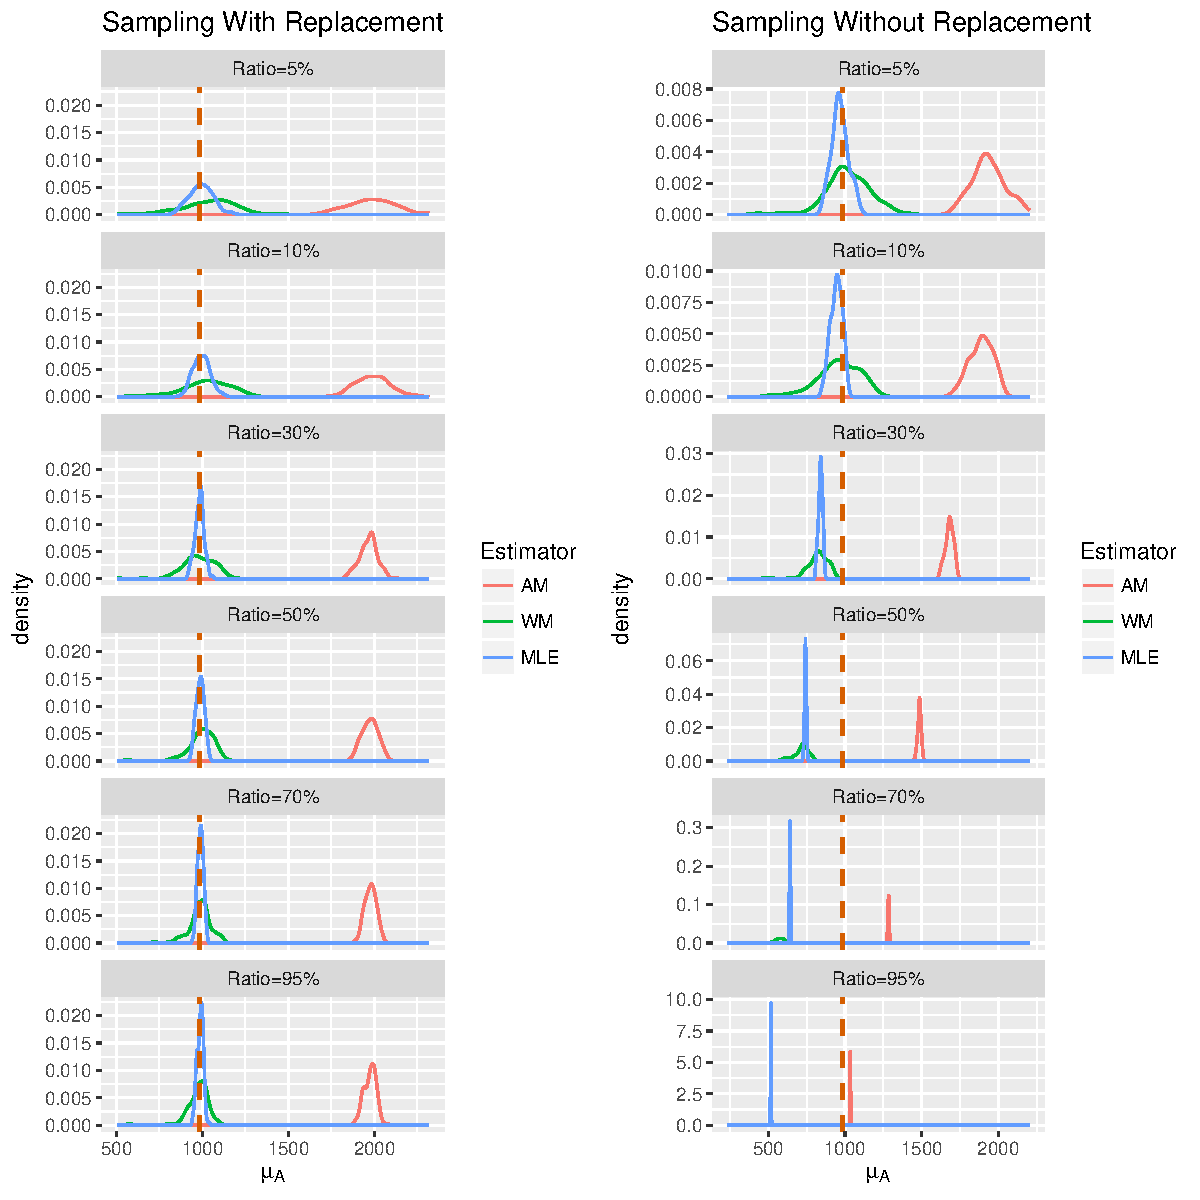
\includegraphics[width=\maxwidth]{figure/unnamed-chunk-3-1} 

\end{knitrout}
  \caption{Sampling Distributions for Area with Different Ratios, N=2000, ${\mu}_{A}$=985.75}
\label{fig_dis_size}
\end{figure}

%latex.default(cbind(t_size_inf, t_size_f), rowname = NULL, file = "",     label = "tab_size_est", col.just = rep(c("c", "c", "r", "r",         "r"), 2), caption.loc = c("bottom"), cgroup = c("Sampling WITH Replacement",         "Sampling WITHOUT Replacement"), caption = "Performance Table for Area",     size = "small")%
\begin{table}[!tbp]
{\small
\begin{center}
\begin{tabular}{ccrrrcccrrr}
\hline\hline
\multicolumn{5}{c}{\bfseries Sampling WITH Replacement}&\multicolumn{1}{c}{\bfseries }&\multicolumn{5}{c}{\bfseries Sampling WITHOUT Replacement}\tabularnewline
\cline{1-11}
\multicolumn{1}{c}{Ratio}&\multicolumn{1}{c}{Estimator}&\multicolumn{1}{c}{Bias}&\multicolumn{1}{c}{Std. Dev.}&\multicolumn{1}{c}{Root MSE}&\multicolumn{1}{c}{}&\multicolumn{1}{c}{Ratio}&\multicolumn{1}{c}{Estimator}&\multicolumn{1}{c}{Bias}&\multicolumn{1}{c}{Std. Dev.}&\multicolumn{1}{c}{Root MSE}\tabularnewline
\hline
5\%&AM&1000&133.9&1000&&5\%&AM&951.12&106.95&951.18\tabularnewline
&WM&45.2&162&47&&&WM&33.71&150.39&35.87\tabularnewline
&MLE&7.1&67&10.8&&&MLE&-17.31&53.47&18.79\tabularnewline
10\%&AM&1003.9&96.3&1003.9&&10\%&AM&903.12&75.07&903.17\tabularnewline
&WM&35&140.4&37&&&WM&-25.54&137.37&28.10\tabularnewline
&MLE&9.1&48.1&11.4&&&MLE&-41.31&37.53&41.76\tabularnewline
30\%&AM&980.2&52.6&980.2&&30\%&AM&696.02&26.21&696.04\tabularnewline
&WM&-8.7&100.6&13.2&&&WM&-163.47&74.31&163.70\tabularnewline
&MLE&-2.8&26.3&5.8&&&MLE&-144.87&13.10&144.91\tabularnewline
50\%&AM&988.4&46&988.5&&50\%&AM&500.30&10.95&500.31\tabularnewline
&WM&11.2&78&14.3&&&WM&-274.76&60.98&274.87\tabularnewline
&MLE&1.3&23&5&&&MLE&-242.73&5.47&242.74\tabularnewline
70\%&AM&991.7&33.2&991.8&&70\%&AM&298.43&3.52&298.43\tabularnewline
&WM&0.9&65.1&8.1&&&WM&-416.20&41.13&416.25\tabularnewline
&MLE&3&16.6&5.1&&&MLE&-343.66&1.76&343.66\tabularnewline
95\%&AM&989.2&34.6&989.2&&95\%&AM&49.93&0.17&49.93\tabularnewline
&WM&-8.9&65&12&&&WM&-697.56&18.23&697.58\tabularnewline
&MLE&1.7&17.3&4.5&&&MLE&-467.91&0.09&467.91\tabularnewline
\hline
\end{tabular}
\caption{Performance Table for Area\label{tab_size_est}}\end{center}}
\end{table}

  
\begin{figure}[!htbp]
  \centering

  \end{figure}


  
\begin{figure}[!htbp]
\centering
\begin{knitrout}
\definecolor{shadecolor}{rgb}{0.969, 0.969, 0.969}\color{fgcolor}
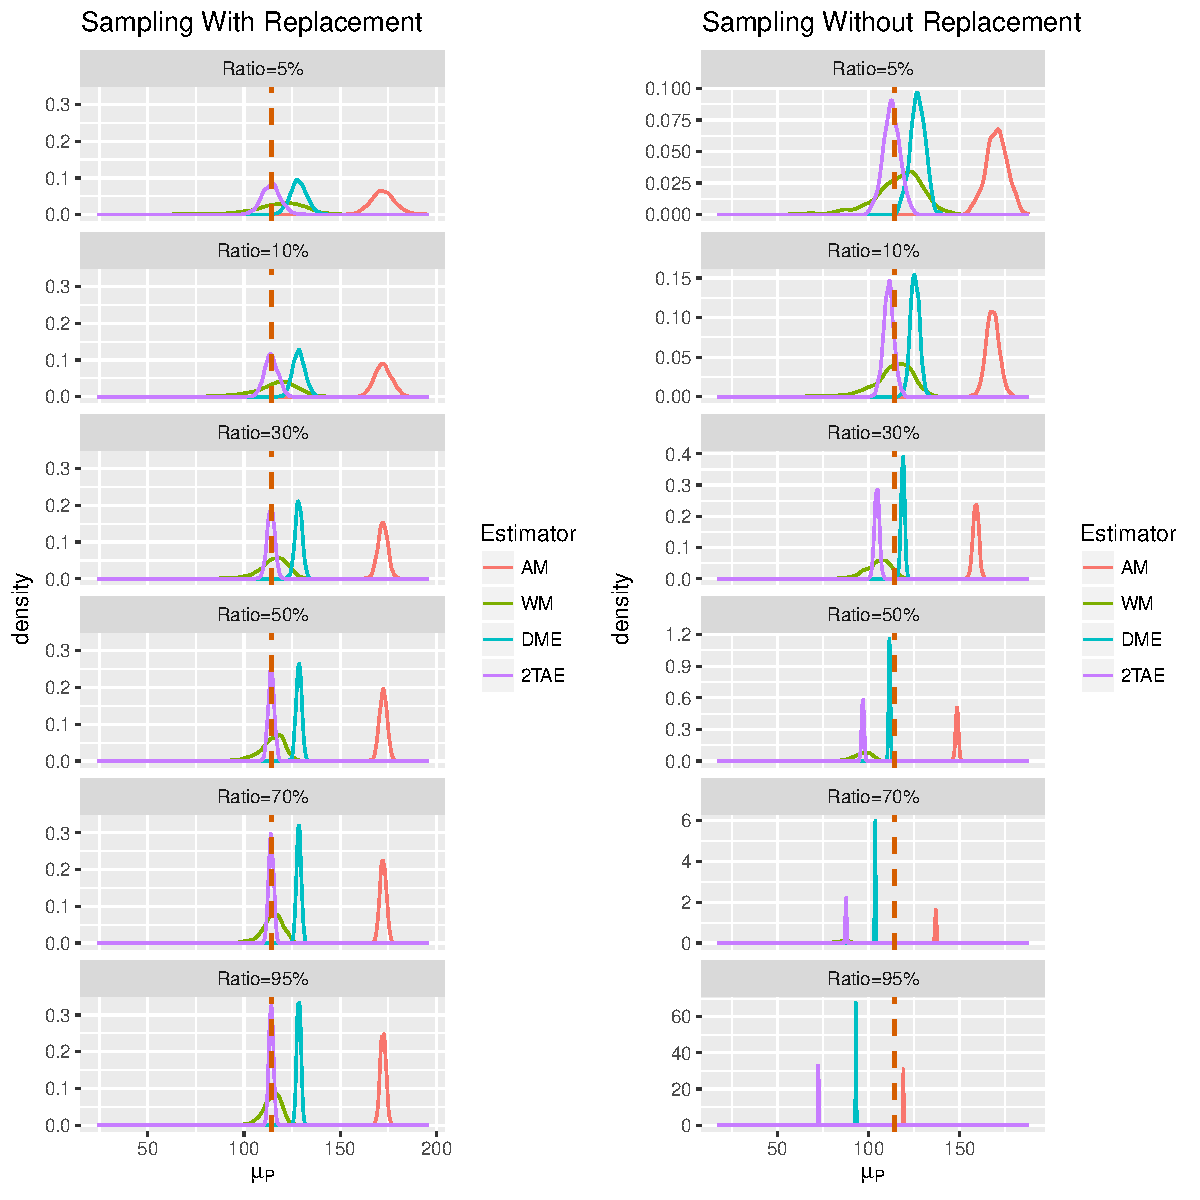
\includegraphics[width=\maxwidth]{figure/unnamed-chunk-7-1} 

\end{knitrout}
  \caption{Sampling Distributions for Perimeter with Different Ratios, N=2000, ${\mu}_{P}$=114.24}  
\label{fig_dis_per}
\end{figure}

%latex.default(cbind(t_per_inf, t_per_f), rowname = NULL, file = "",     col.just = rep(c("c", "c", "r", "r", "r"), 2), caption.loc = c("bottom"),     label = "tab_per_est", cgroup = c("Sampling WITH Replacement",         "Sampling WITHOUT Replacement"), caption = "Performance Table for Perimeter",     size = "footnotesize")%
\begin{table}[!tbp]
{\footnotesize
\begin{center}
\begin{tabular}{ccrrrcccrrr}
\hline\hline
\multicolumn{5}{c}{\bfseries Sampling WITH Replacement}&\multicolumn{1}{c}{\bfseries }&\multicolumn{5}{c}{\bfseries Sampling WITHOUT Replacement}\tabularnewline
\cline{1-11}
\multicolumn{1}{c}{Ratio}&\multicolumn{1}{c}{Estimator}&\multicolumn{1}{c}{Bias}&\multicolumn{1}{c}{Std. Dev.}&\multicolumn{1}{c}{Root MSE}&\multicolumn{1}{c}{}&\multicolumn{1}{c}{Ratio}&\multicolumn{1}{c}{Estimator}&\multicolumn{1}{c}{Bias}&\multicolumn{1}{c}{Std. Dev.}&\multicolumn{1}{c}{Root MSE}\tabularnewline
\hline
5\%&AM&58.05&6.30&58.11&&5\%&AM&55.95&5.80&56.01\tabularnewline
&WM&2.93&15.81&4.94&&&WM&1.64&14.76&4.18\tabularnewline
&DME&14.23&4.43&14.38&&&DME&12.70&4.07&12.86\tabularnewline
&2TAE&-0.10&4.91&2.22&&&2TAE&-1.63&4.57&2.69\tabularnewline
10\%&AM&58.12&4.42&58.16&&10\%&AM&53.79&3.58&53.82\tabularnewline
&WM&1.87&12.25&3.97&&&WM&-0.87&11.71&3.53\tabularnewline
&DME&14.34&3.15&14.45&&&DME&11.17&2.47&11.28\tabularnewline
&2TAE&-0.07&3.44&1.85&&&2TAE&-3.15&2.85&3.58\tabularnewline
30\%&AM&57.94&2.59&57.96&&30\%&AM&44.61&1.56&44.62\tabularnewline
&WM&0.72&8.82&3.06&&&WM&-9.35&7.53&9.75\tabularnewline
&DME&14.24&1.86&14.31&&&DME&4.55&0.98&4.65\tabularnewline
&2TAE&-0.22&2.00&1.43&&&2TAE&-9.66&1.31&9.73\tabularnewline
50\%&AM&58.17&2.02&58.19&&50\%&AM&34.24&0.76&34.25\tabularnewline
&WM&0.42&6.32&2.55&&&WM&-17.78&5.69&17.94\tabularnewline
&DME&14.39&1.45&14.44&&&DME&-2.76&0.43&2.84\tabularnewline
&2TAE&-0.04&1.56&1.25&&&2TAE&-17.38&0.66&17.39\tabularnewline
70\%&AM&58.09&1.65&58.10&&70\%&AM&22.60&0.35&22.61\tabularnewline
&WM&0.42&5.90&2.46&&&WM&-28.71&4.66&28.79\tabularnewline
&DME&14.33&1.18&14.37&&&DME&-10.61&0.17&10.62\tabularnewline
&2TAE&-0.10&1.29&1.14&&&2TAE&-26.65&0.31&26.65\tabularnewline
95\%&AM&58.09&1.47&58.11&&95\%&AM&4.85&0.05&4.85\tabularnewline
&WM&0.38&5.18&2.31&&&WM&-58.41&2.85&58.44\tabularnewline
&DME&14.33&1.05&14.36&&&DME&-21.19&0.02&21.19\tabularnewline
&2TAE&-0.09&1.13&1.07&&&2TAE&-41.83&0.03&41.83\tabularnewline
\hline
\end{tabular}
\caption{Performance Table for Perimeter\label{tab_per_est}}\end{center}}
\end{table}

  

\end{document}
